%%%%%%%%%%%%%%%%%%%%%%%%%%%%%%%%%%%%%%%%%
% fphw Assignment
% LaTeX Template
% Version 1.0 (27/04/2019)
%
% This template originates from:
% https://www.LaTeXTemplates.com
%
% Authors:
% Class by Felipe Portales-Oliva (f.portales.oliva@gmail.com) with template 
% content and modifications by Vel (vel@LaTeXTemplates.com)
%
% Template (this file) License:
% CC BY-NC-SA 3.0 (http://creativecommons.org/licenses/by-nc-sa/3.0/)
%
%%%%%%%%%%%%%%%%%%%%%%%%%%%%%%%%%%%%%%%%%

%----------------------------------------------------------------------------------------
%	PACKAGES AND OTHER DOCUMENT CONFIGURATIONS
%----------------------------------------------------------------------------------------

\documentclass[
	12pt, % Default font size, values between 10pt-12pt are allowed
	%letterpaper, % Uncomment for US letter paper size
	%spanish, % Uncomment for Spanish
]{fphw}

% Template-specific packages
\usepackage[utf8]{inputenc} % Required for inputting international characters
\usepackage[T1]{fontenc} % Output font encoding for international characters
\usepackage{mathpazo} % Use the Palatino font
\usepackage{setspace}

\usepackage{graphicx} % Required for including images

\usepackage{booktabs} % Required for better horizontal rules in tables

\usepackage{listings} % Required for insertion of code

\usepackage{enumerate} % To modify the enumerate environment

\usepackage{parskip}% http://ctan.org/pkg/parskip

\usepackage{amsmath}

\usepackage{amssymb}

\usepackage{caption}

\usepackage{tikz}
\newcommand*\circled[1]{\tikz[baseline=(char.base)]{
            \node[shape=circle,draw,inner sep=2pt] (char) {#1};}}

            \usetikzlibrary{decorations.pathreplacing,positioning, arrows.meta}

            \newcommand{\ImageWidth}{\textwidth}

\usepackage{enumitem}

\usepackage[ruled,portuguese,onelanguage,longend]{algorithm2e} %for psuedo code}% http://ctan.org/pkg/algorithm2e
% \makeatletter
% \renewcommand{\@algocf@capt@plain}{above}% formerly {bottom}
% \makeatother

%----------------------------------------------------------------------------------------
%	ASSIGNMENT INFORMATION
%----------------------------------------------------------------------------------------

\title{AULA 10 - Instrumentação} % Assignment title

\author{AVC, JPP, PC} % Student name

\date{} % Due date

\institute{Pontifícia Universidade Católica do Rio de Janeiro \\ Departamento de Informática} % Institute or school name

\class{Programação Modular (INF1301)} % Course or class name

\professor{Flavio Bevilacqua} % Professor or teacher in charge of the assignment

%----------------------------------------------------------------------------------------

\begin{document}

\maketitle % Output the assignment title, created automatically using the information in the custom commands above

%----------------------------------------------------------------------------------------
%	ASSIGNMENT CONTENT
%----------------------------------------------------------------------------------------
\begin{doublespace}

    \begin{enumerate}[label=\textbf{\arabic*})]

        \item \textbf{Problema ao realizar testes}

              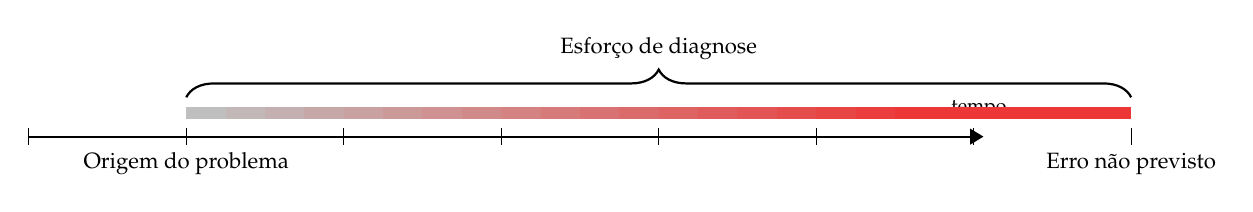
\begin{tikzpicture}
                  % draw horizontal line   
                  \draw[thick, -Triangle] (0,0) -- (\ImageWidth,0) node[font=\scriptsize,above left=3pt and -12pt]{tempo};

                  % draw vertical lines
                  \foreach \x in {0,1,...,7}
                  \draw (\x *2cm,3pt) -- (\x *2cm,-3pt);

                  \foreach \x/\descr in {2/$Origem do problema$, 14/$Erro não previsto$}
                  \node[font=\footnotesize, text height=1.75ex,
                      text depth=.5ex] at (\x,-.3) {$\descr$};

                  % colored bar up
                  \foreach \x/\perccol in
                      {2/100,2.5/96,3/92,3.5/88,4/84,4.5/80,5/76,5.5/72,6/68,6.5/64,7/60,7.5/56,8/52,8.5/48,9/44,9.5/40,10/36,10.5/32,11/28}
                  \draw[lightgray!\perccol!red, line width=4pt]
                  (\x,.3) -- +(3,0);
                  %   \draw[-Triangle, dashed, red] (5,.5) --  +(1,0);

                  % braces
                  \draw [thick ,decorate,decoration={brace,amplitude=10pt}] (2,0.5)  -- +(12,0)
                  node [black,midway,above=10pt, font=\footnotesize] {Esforço de diagnose};

              \end{tikzpicture}

              Colocamos controles ao longo do processo de desenvolvimento para minimizar o esforço de diagnose. Com controles, sabemos até qual ponto a aplicação estava correta e minimizamos possibilidades de erros.

              Esforço de diagnose

              \begin{itemize}

                  \item Grande
                  \item Muito sujeito a erros

              \end{itemize}

              Contribui para esta dificuldade (agravantes)

              \begin{itemize}

                  \item Não estabelece com facilidade a origem do problema.
                  \item Tempo decorrido entre o instante da falha e o observado.
                  \item Falhas intermitentes, acontecem de vez em quando.
                  \item Causa externa ao código, falhas não relacionadas ao código da aplicação.

              \end{itemize}

        \item \textbf{O que é Instrumentação?}

              Instrumentação são fragmentos de código de controle inseridos na aplicação durante o desenvolvimento de forma a monitorar a execução e minimizar o esforço de diagnose. Fragmentos de código de controle podem ser dados (redundantes) ou comandos (blocos de controle). Eles não contribuem para o objetivo do programa, consomem recursos de execução e custam para serem desenvolvidos.

        \item \textbf{Objetivos}

              \begin{itemize}

                  \item Detectar falhas de funcionamento do programa o mais cedo possível de forma automática.
                  \item Impedir que falhas se propaguem.
                  \item Medir propriedades dinâmicas do programa.

              \end{itemize}

        \item \textbf{Conceitos}

              \begin{itemize}

                  \item Programa robusto: intercepta a execução quando observa o problema e mantém o dano confinado.
                  \item Programa tolerante a falhas: é robusto e possui mecanismo de recuperação, ou seja, o programa é preparado para condição hostil do ambiente (Ex: permite salvar progresso quando encontra erro).
                  \item Deteriorização controlada: programa recupera de uma instabilidade e continua funcionando mesmo com uma perda de funcionalidade (subconjunto de tolerância a falhas).
                  \item Esquema de inclusão de instrumentos em C e C++:

                        % Todo trecho de instrumentação fica antre \#ifdef _DEBUG e \#endif

                        % \#ifdef _DEBUG
                        % - codigos
                        % - dados
                        % \#endif

              \end{itemize}

        \item \textbf{Assertivas Executáveis}

              Assertivas se tornam código para testá-las. Assertivas precisam ser corretas e completas. Vantagens: informa um problema quase imediatamente após ter sido gerado, controle de integridade é feito pela máquina, reduz o risco de falha humana.

    \end{enumerate}


\end{doublespace}
%----------------------------------------------------------------------------------------

\end{document}
